\setchapterimage[7cm]{ztf_telescope.png}
\chapter{The Zwicky Transient Facility}
\labch{ZTF}
The second instrument relevant for this thesis is the Zwicky Transient Facility (ZTF). It is named after the notorious Swiss-American astronomer Fritz Zwicky, who e.g. first employed the Virial theorem to infer the existence of dark matter \sidecite{Zwicky1933}. Furthermore, together with Walter Baade, he posited the existence of supernovae and the creation of neutron stars in such events \sidecite{Baade1934}.

ZTF is a wide-field optical survey telescope. This means that it normally operates by scanning the full sky with a fixed cadence, in contrast to pointing to specific objects. It is located at Mount Palomar in California, United States, at \SI{1700}{\m} above sea level, roughly \SI{130}{\km} southeast of Los Angeles. Its optical system, the \SI{1.2}{\m} (48 inch) Samuel Oschin telescope, is a Schmidt design (see below) and was inaugurated in 1948 \cite{Harrington1952}. At the time of inauguration and for years to come, it was the largest Schmidt telescope in the world. Originally, the telescope used photographic plates, covering a field of view (FoV) of \SI{44}{\square\deg}. As these have obvious drawbacks, and because technological progress made it possible, the Near-Earth Asteroid Tracking (NEAT) program \sidecite{Pravdo1999} replaced the photographic plates with a charge-coupled device (CCD) camera in the early 2000s.\marginnote{See \url{https://sites.astro.caltech.edu/palomar/about/telescopes/oschin.html} for a historical overview.}

The camera was updated several times over the course of the next years. The immediate predecessor of ZTF, the Palomar Transient Factory (PTF) \sidecite{Law2009}, began operation in 2009. Equipped with a 96 Megapixel camera, it already had many of the characteristics of ZTF: A fully automated survey, searching for optical transients with a CCD camera.

PTF's successor in spirit, ZTF, contains the first electronic camera. With \SI{47}{\square\deg}, it covers almost the full FoV of the P48. The main design metric for ZTF was \textit{volumentric survey speed} \sidecite{Bellm2016}. This is the volume within which an object of given absolute magnitude can be detected in one exposure, divided by the total time for the exposure (observation plus overhead). The system saw first light in 2017, and started its scientific use in the year after. As of writing, it is still operational.

The two other telescopes located on Mount Palomar. The \SI{1.5}{\meter} (60 inch) P60 telescope houses the SED Machine (SEDM) \sidecite{Blagorodnova2018}, a fully robotic, low-resolution spectrograph used for automatic classification of transients. The largest facility on the mountain is the 200-inch (\SI{5.1}{\meter}) Hale Telescope, which is used for optical and infrared photometry as well as mid- and high-resolution spectroscopy of fainter sources. Together, these telescopes form a natural hierarchy: ZTF is the discovery engine for optical transients. Promising sources are then classified with SEDM. If sources warrant it, deeper photometry and higher resolved spectroscopy can then be obtained with the big gun, the P200. All three telescopes are shown in Fig. \ref{fig:palomar_overview}.

\begin{figure*}[]
    \includegraphics{palomar_overview}
    \caption[View of Mt. Palomar]{View of Mt. Palomar with the three telescopes highlighted in the text. Image credit: Caltech, annotations added by the author.}
    \labfig{palomar_overview}
\end{figure*}

\section{Telescope Design}
A \textit{Schmidt telescope} is by design dedicated to taking images, contrary to earlier designs allowing actually looking through an eyepiece \sidecite{Schmidt1938}. For this reason, it is also referred to as a \textit{Schmidt camera}. The design goal is a wide FoV. This makes it the ideal instrument for sky surveys, where a large FoV maximizes the on-sky area that can be monitored. A Schmidt telescope combines a spherical mirror at the end of the telescope tube with an aspherical correcting lens (Schmidt plate) at the tube's entrance. The use of a spherical mirror combined with the correcting lens gets entirely rid of comatic aberration.

\begin{figure}[]
    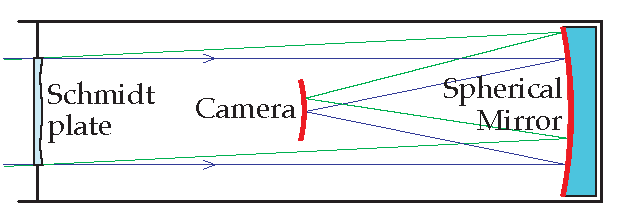
\includegraphics[width=1\textwidth]{schmidt2.pdf}
    \caption[Schmidt telescope schematic]{Schmidt telescope schematic. Light enters from the left, passes the Schmidt plate (an aspherical correcting lens), gets reflected by a spherical mirror at the end onto a photographic plate or camera halfway down the tube. Figure adopted from \url{https://commons.wikimedia.org/wiki/File:Schmidt-Teleskop.svg}.}
    \labfig{schmidt_telescope}
\end{figure}

Until the end of the 20th century, around ten Schmidt telescopes have been built, most of them to conduct sky surveys \sidecite{Cannon1995}. At least two of them were space telescopes: ESA's astrometry mission \textit{HIPPARCOS} \sidecite{ESA1997} (1989--1993) and the NASA explanet mission \textit{Kepler} \sidecite{Koch2010} (2009--2018). In both cases, the mission entailed monitoring of large areas of the sky; prime territory for Schmidt telescopes.

\begin{figure}[]
    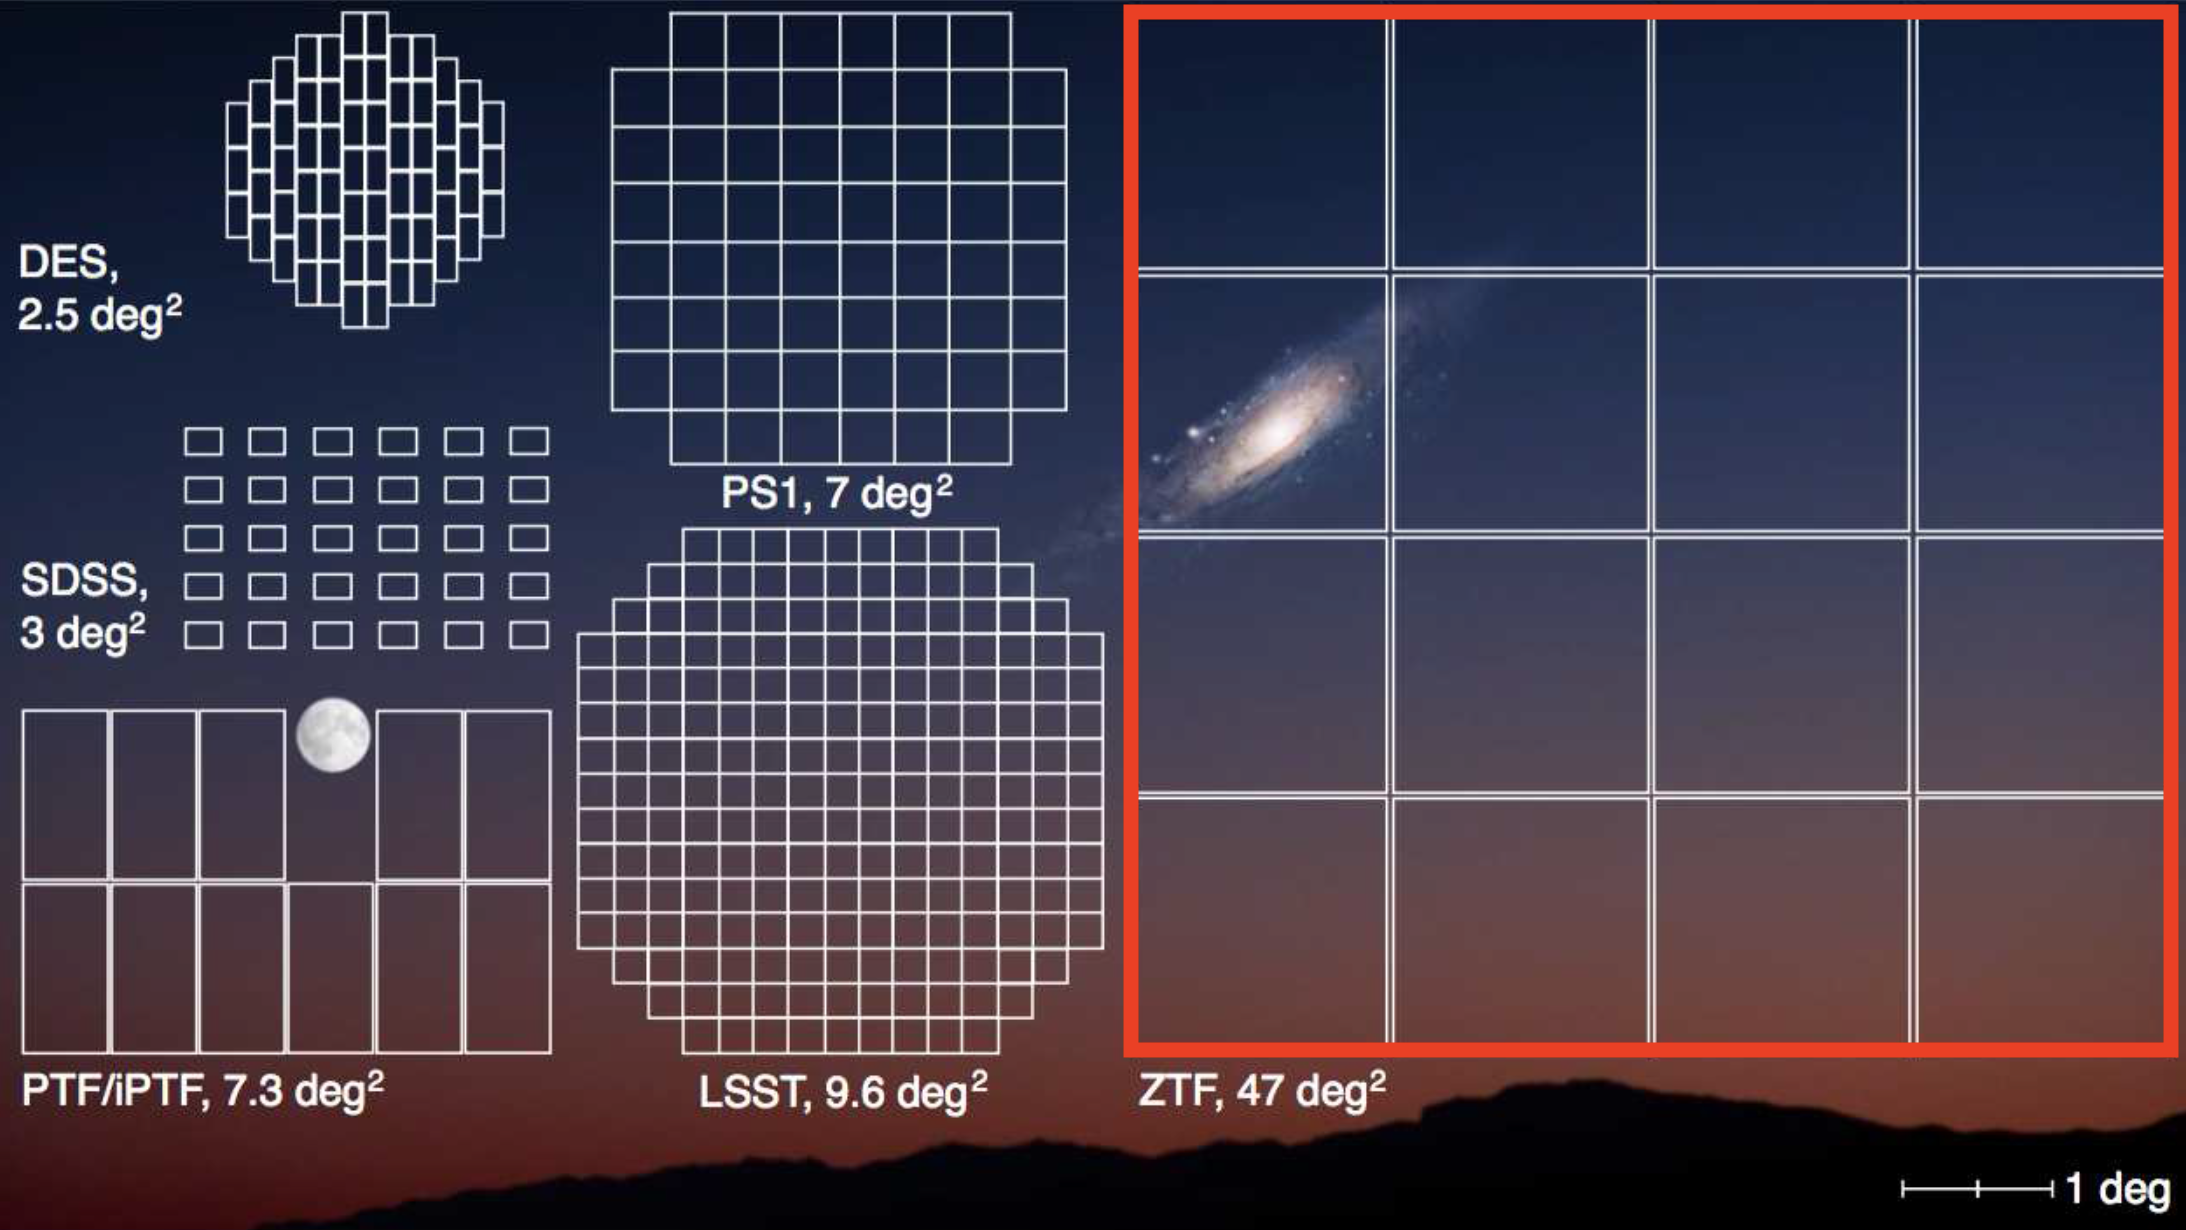
\includegraphics[width=1\textwidth]{ztf_fov.png}
    \caption[ZTF Field of View]{ZTF field of view (highlighted in red) in comparison to other sky survey telescopes, including the future Rubin observatory (LSST). Note also the 6.5-fold increase with respect to ZTF's predecessor, PTF/iPTF. From \cite{Laher2018}, highlighting by the author.}
    \labfig{ztf_fov}
\end{figure}



\section{Camera}
The ZTF camera is a CCD design, consisting of 16 individual CCDs by commercial manufacturer e2v (now Teledyne, \textit{Science CCD231-C6}), each having 6144x6160 pixels, resulting in a total camera resolution of $\sim 600 \,\textrm{Megapixel}$ \sidecite{Dekany2016}. As one can see in Fig. \ref{fig:ztf_camera}, the array of 16 CCDs is slightly bent. This is necessitated by the Schmidt design, where the camera needs to be spherical, matching the spherical mirror. As individual CCDs are flat, each of the 16 sensors is is installed slightly tilted, tracing the overall curvature. To get rid of residual deviations from the global curvature, in front of each sensor a field flattener lens is mounted \sidecite{Bellm2019}.

\begin{marginfigure}
    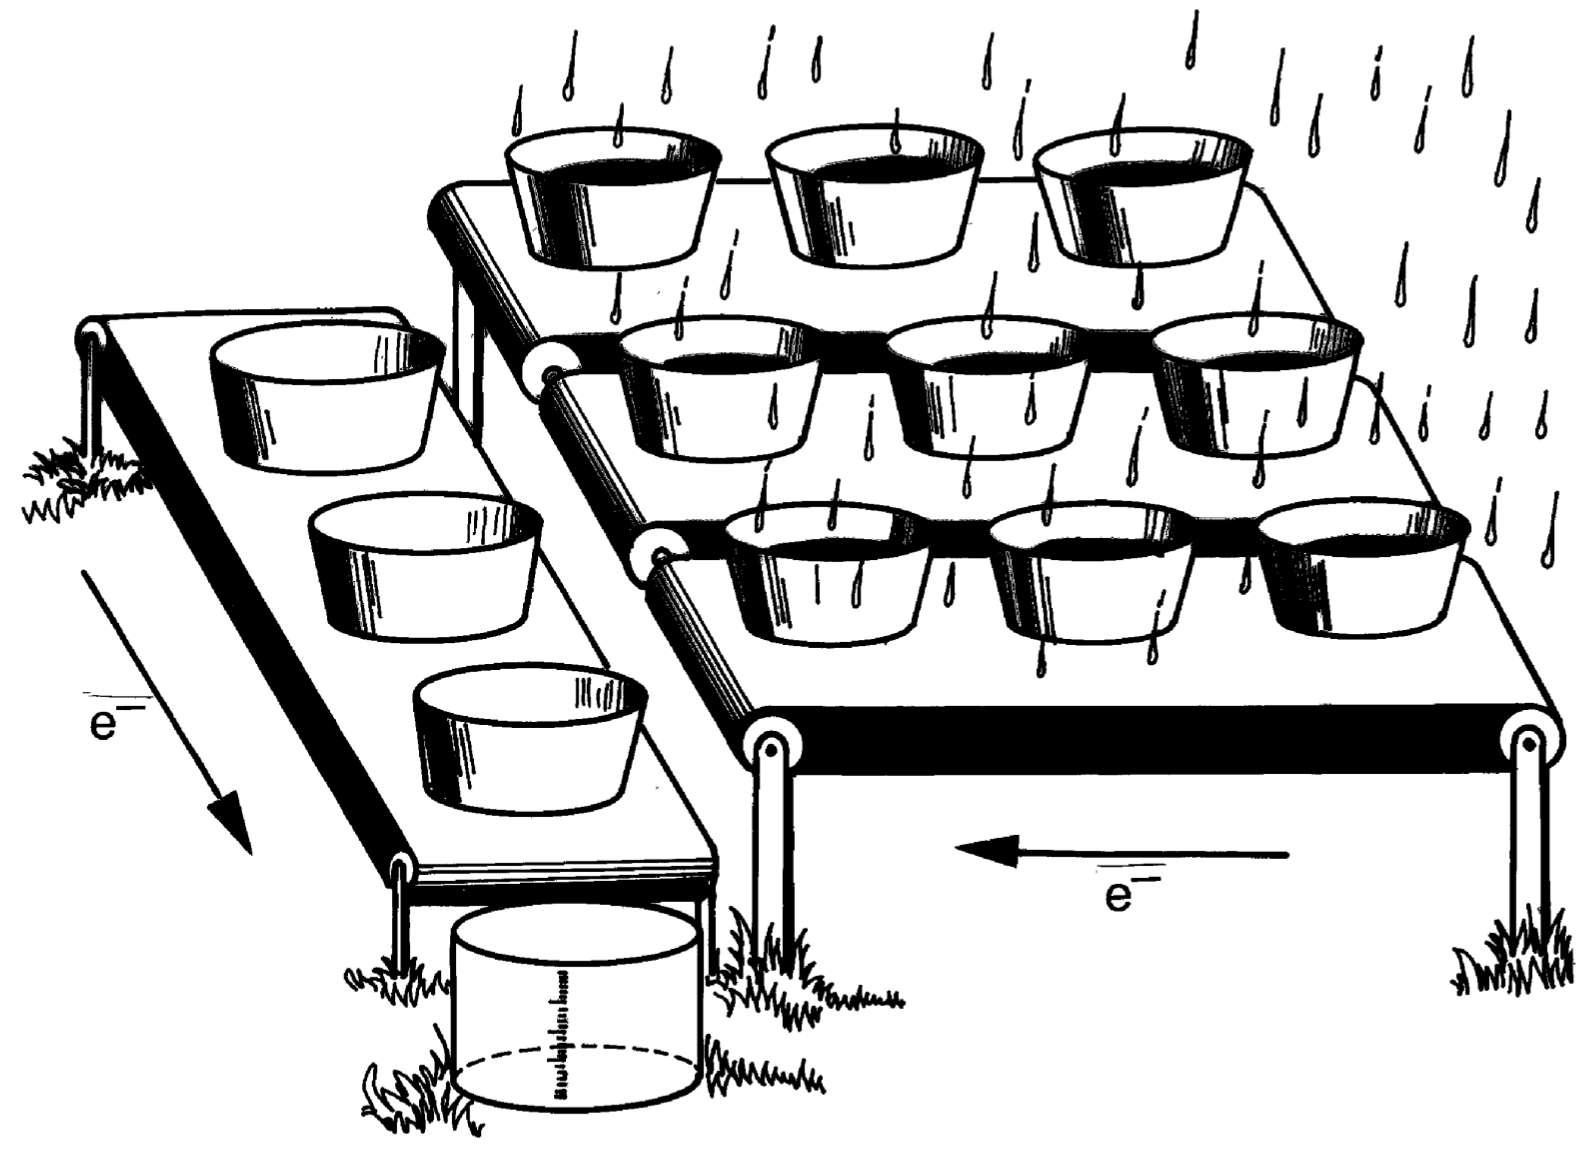
\includegraphics{ccd_buckets.png}
    \caption[CCD operational principle]{CCD operational principle, explained with buckets measuring precipitation. From \cite{Janesick1987}.}
    \labfig{ccd_buckets}
\end{marginfigure}

\subsection*{CCDs}
CCDs are silicon-based light sensors. They consist of arrays of coupled metal-oxide semiconductor (MOS) capacitors, each one able to store the charge created by incident photons; one capacitor per pixel of the sensor array. The array is exposed to light for an amount of time (exposure time). During the exposure, incident photons create a charge proportional to the amount of light hitting each capacitor via the photo-electric effect. This charge is accumulated in each capacitor until the exposure is finished. To read out the CCD, the charges need to be moved to neighboring capacitors. When the MOS capacitors are tightly placed, one can move the charges from one capacitor to the next by changing the voltages on the capacitor's gates.

In Fig. \ref{fig:ccd_buckets} the principle of a CCD is explained with little buckets collecting rain water. Each bucket symbolizes one capacitor or one pixel of the sensor array respectively. After the rain has stopped (the exposure is finished), each bucket naturally contains an amount of water proportional to the amount of water that rained down over it. Now the amount of water in each bucket (the charge deposited by incident light in each capacitor) needs to be measured.

To do this, the buckets in each row are moved one position to the left with horicontal conveyor belts. Each bucket at the left end of the horicontal conveyor belt is then emptied into the bucket on the single vertical conveyor belt. The buckets of this vertical belt are then one by one drained into the meausuring bucket on the bottom left. After all buckets on the vertical belt are emptied, the process starts anew, until all buckets are empty. As one can see, the time this process takes scales linearly with the amount of buckets (or pixels) \sidecite{Janesick1987}. To speed up the process, one can subdivide the sensor area into smaller sections, which are read out in parallel.

\begin{marginfigure}
    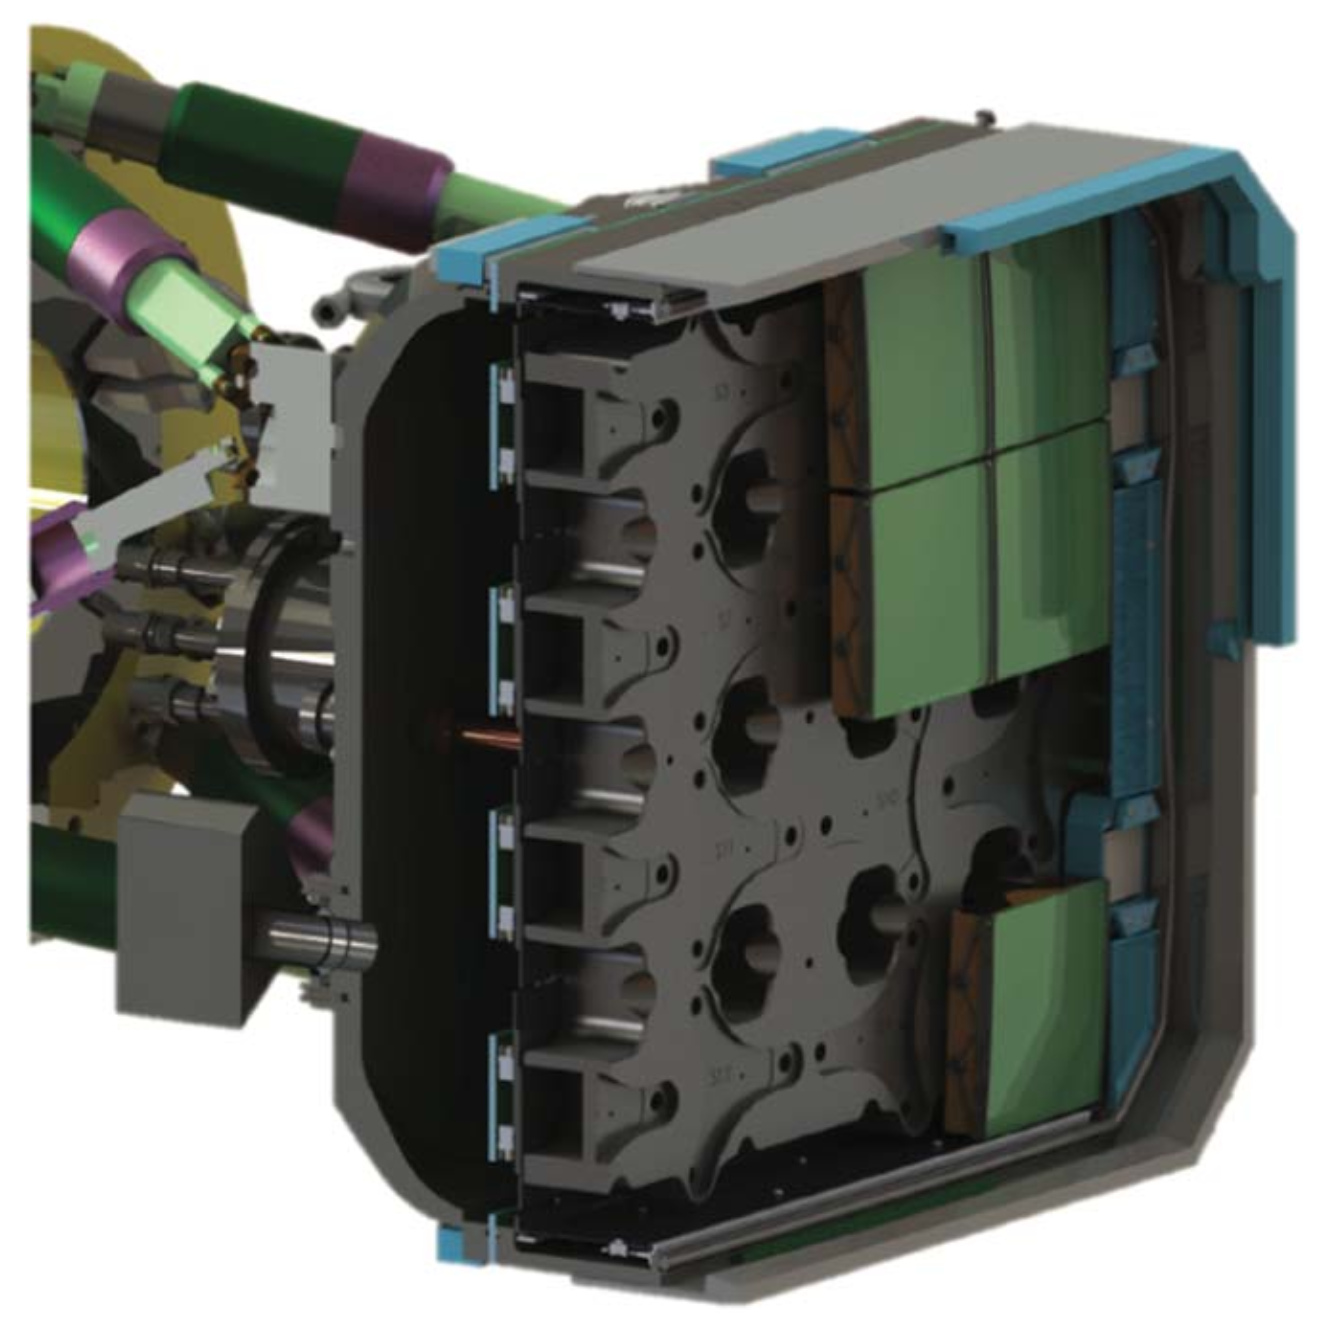
\includegraphics{ztf_camera_detail.png}
    \caption[ZTF camera cutaway]{The ZTF camera in detail. From \cite{Dekany2020}.}
    \labfig{ztf_camera_detail}
\end{marginfigure}

The typical exposure for the ZTF camera is \SI{30}{\second}, while the readout time (emptying and measuring the charges in each capacitor) takes \SI{8.2}{\second}. Readout and digitization is done in parallel for four quadrants, each containing 4 CCDs. The four readout devices for the quadrants are \textit{Archon} CCD controllers by Semiconductor Technology Associates (STA). Each of these operates 16 simultaneous readout channels, four for each CCD. In summary, the camera is read out simultaneously in 64 independent regions to speed up the process.

An additional four smaller CCDs (2k x 2k pixels) are used as guidance, tip, tilt and focus sensors, with one additional Archon controller to read out these sensors \sidecite{Dekany2020}. To lower the thermal noise of the camera, it is placed on top of a cryostat cooling the CCDs to \SI{160}{\kelvin} \cite{Dekany2016}.

\begin{figure}[t!]
    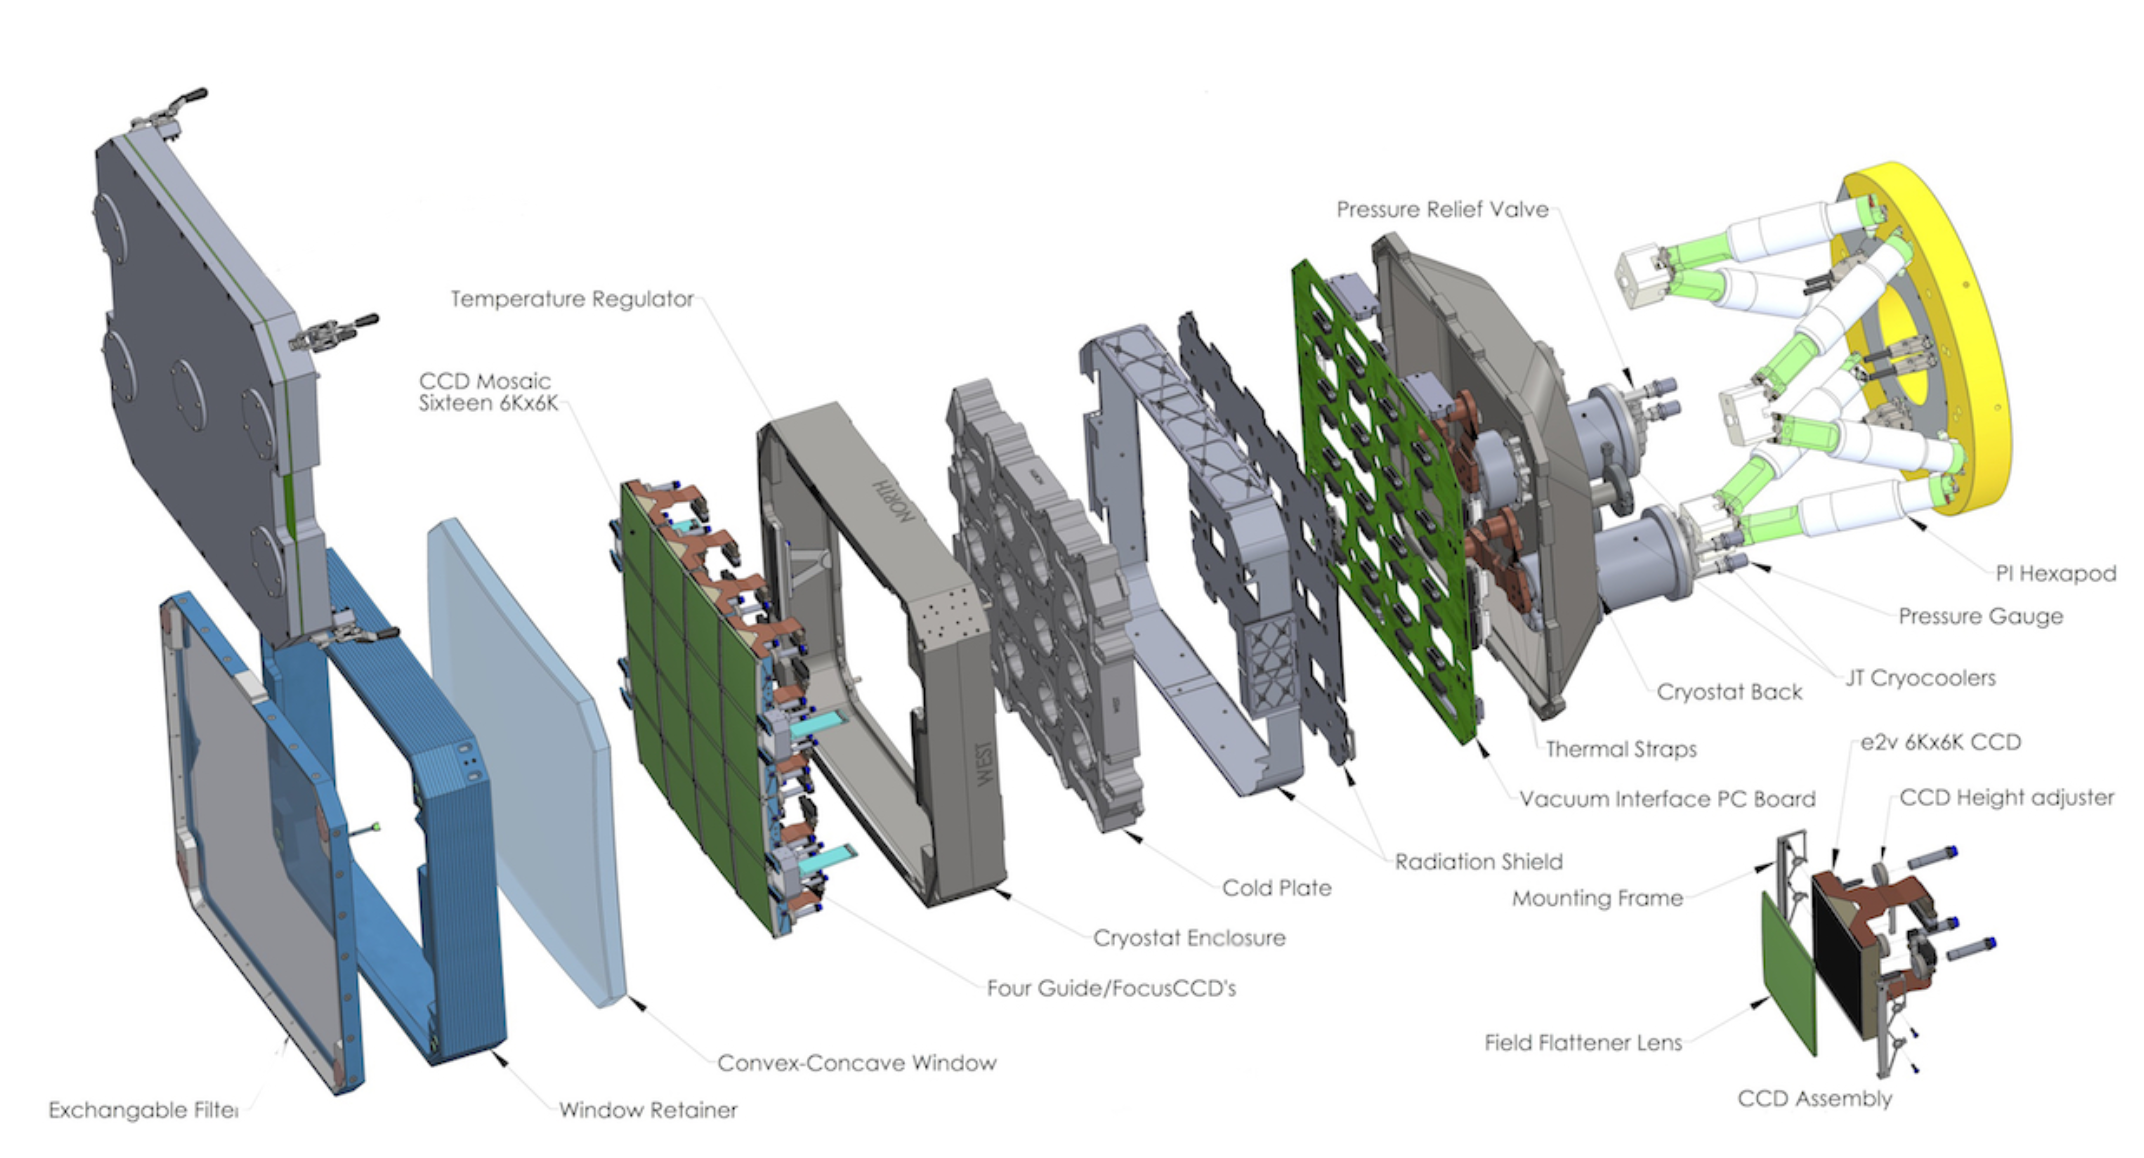
\includegraphics[width=1\textwidth]{ztf_camera.png}
    \caption[ZTF cmera]{The ZTF camera. One can see the CCDs sandwiched between the filter on the front and the cryostat on the back. From \cite{Bellm2019}.}
    \labfig{ztf_camera}
\end{figure}

\section{Optical System}

\subsection*{Filters and shutter}
As the CCDs of the camera cannot ``see'' color, different filters need to be put in front of the camera to obtain color information. With ZTF, there are three different filters available: A \textit{g}-band filter with a median wavelength of \SI{472}{\nano \meter} (corresponding to blue light), an \textit{r}-band filter (median wavelength: \SI{634}{\nano \meter}, red light) and an \textit{i}-band filter (\SI{789}{\nano \meter}, near-infrared). These filters can be changed with a robotic arm, securely stowing the replaced filter and magnetically attaching the new one \cite{Dekany2020}. This process takes \SI{110}{\second} \cite{Bellm2019}. 

The main decision goal for the filter selection was to the maximize signal-to-noise ratio by avoiding major sky emission lines at Mt. Palomar while avoiding excessive costs. ZTF does not exactly match the filters of potential calibrators, e.g. the Sloan Digital Sky Survey (SDSS) \sidecite{York2000}, PanSTARRS (PS1) \sidecite{Kaiser2002} or \textit{Gaia} \sidecite{Prusti2016}. This was justified with the overall different telescope design of ZTF \cite{Bellm2019}.

\begin{marginfigure}
    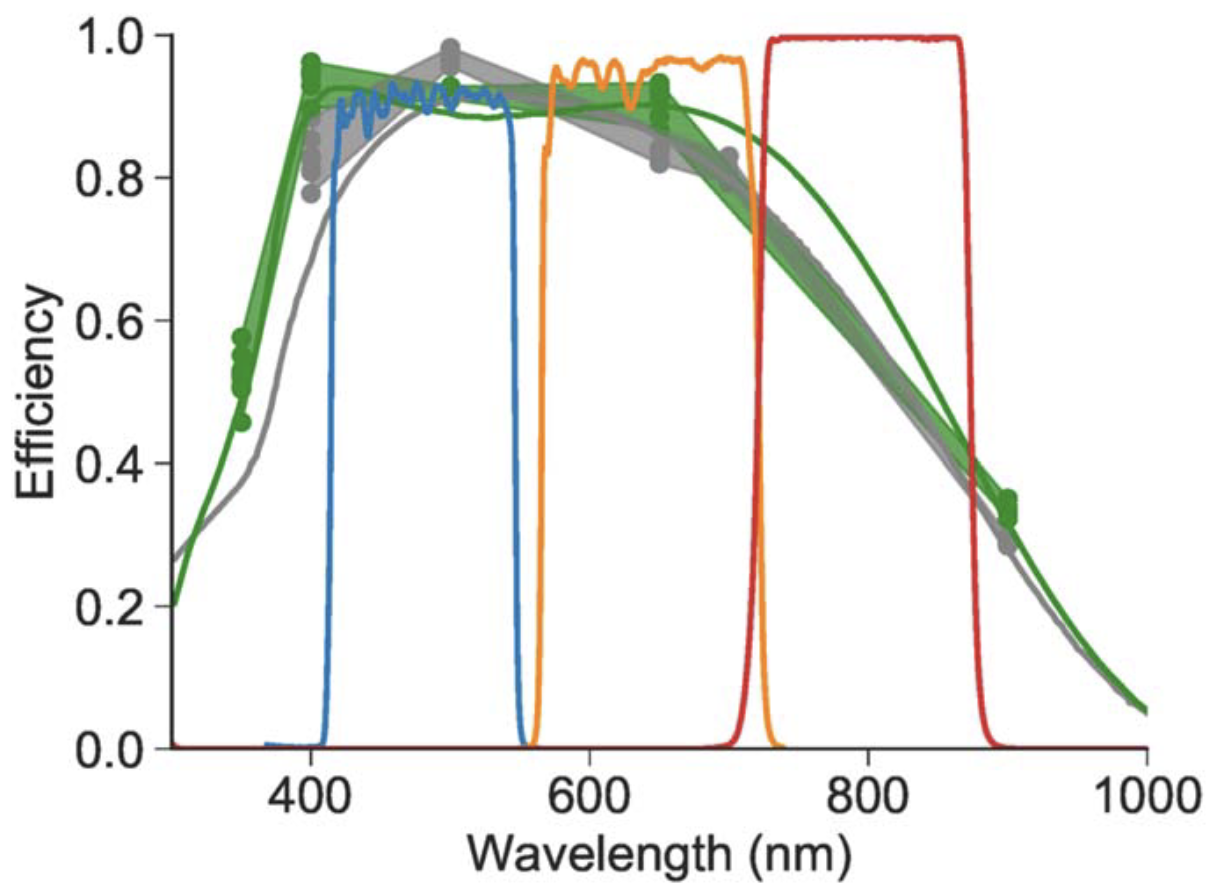
\includegraphics{ztf_throughput.png}
    \caption[ZTF filter transmission]{ZTF filter transmission for the three different bands (\textit{g}-band: blue, \textit{r}-band: orange, \textit{i}-band: red). The green and gray datapoints show the CCD quantum efficiency measurements (single and double-layer reflective coating). From \cite{Bellm2019}.}
    \labfig{ztf_transmission}
\end{marginfigure}

The transmission of each filter and the CCD quantum efficiency curve can be seen in Fig. \ref{fig:ztf_transmission}. As one can see, the quantum efficiency starts to decrease within the \textit{r}-band towards higher wavelengths, rendering the \textit{i}-band the least sensitive of the three filters. The $5\sigma$ median sensitivity for a 30s exposure reflects that fact. It is 20.8 (21.1) mag in the \textit{g}-band, 20.6 (20.9) mag in the \textit{r}-band and 19.9 (20.2) mag in the \textit{i}-band; with values for optimal conditions (new moon) in brackets. The resulting median image quality is 2.1'' (\textit{g}-band), 2.0'' (\textit{r}-band) and 2.1'' full width at half maximum (FWHM) of the point spread function (PSF, see \nameref{psfphot} section below) \cite{Bellm2019}.

To decrease light obstruction, the ZTF shutter was newly developed and is mounted in front of the aperture, outside of the telescope tube. It was developed by Deutsches Elektronen-Synchrotron (DESY) in cooperation with industry partner Bonn-Shutter and allows to open and close in \SI{290}{\milli \second} \cite{Dekany2020}.

\subsection*{ZTF grid} \label{ztf_grid}
One exposure during regular operations -- in contrast to e.g. deep target of opportunity (ToO) images -- lasts \SI{30}{\second}. There is an additional \SI{\sim 15}{\second} overhead for readout and slewing the telescope. Also some additional time is needed to exchange the filters. Therefore, a typical night lasting \SI{8.67}{\hour} \sidecite{Masci2019} results in roughly 700 exposures. In total, these amount to a sky area of over \SI{32500}{\square\deg}, allowing to cover the full visible sky at Mount Palomar \SI{15}{\degree} above the horizon at least once.

\begin{marginfigure}
    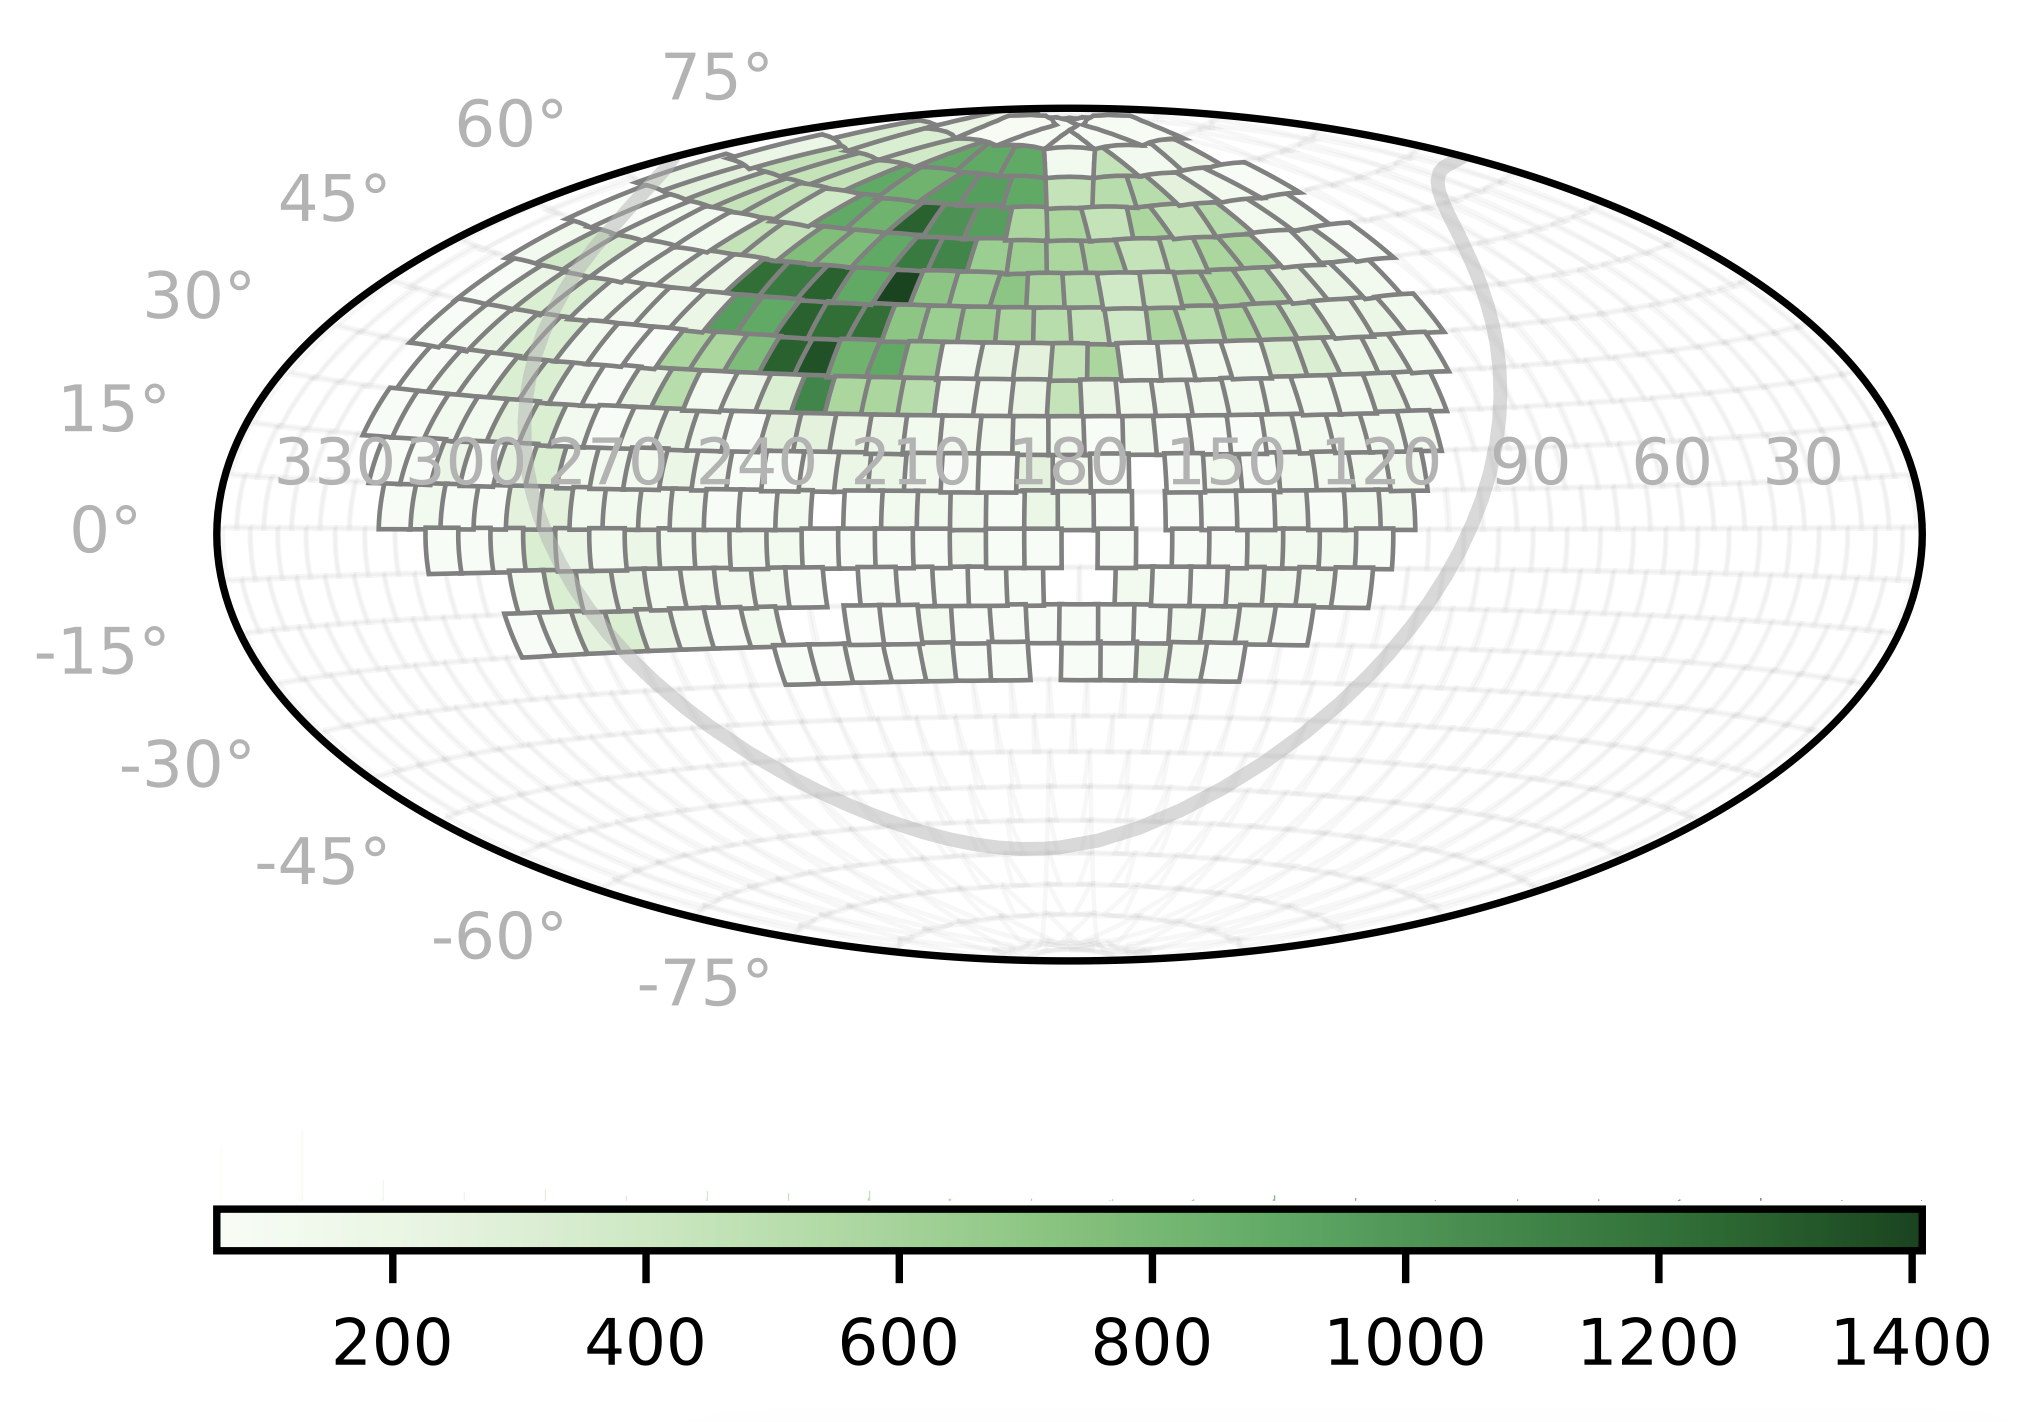
\includegraphics{ztf_g_band_grid}
    \caption[ZTF field visits]{Number of ZTF \textit{g}-band field visits during the first week of May 2020. The primary grid fully tiles the sky accessible at Mount Palomar.}
    \labfig{ztf_g_field_visits}
\end{marginfigure}

To aid in the robotic operation and to simplify matters, ZTF operates on a fixed primary on-sky grid of so-called ``fields''. Each field corresponds to a fixed sky location with an area of \SI{47}{\square\deg}, and the telescope is exclusively pointing to those fields. Note that with such a system, some parts of the sky will always fall into the chip gaps (the parts of the FoV that fall between the 16 CCDs). To mitigate that, there exists a \textit{secondary grid} that is diagonally offset from the primary grid. Fig. \ref{fig:ztf_g_field_visits} shows the primary grid and the number of visits per field in the \textit{g}-band during the first week of May 2020.

\section{Calibration and Image Processing}
The ZTF image processing can be divided into two parts: Creation of the science exposures takes places locally at Mount Palomar, while calibration, creation of the final data products, extraction of transients and archival storage happens at the Infrared Processing and Analysis Center (IPAC)\sidenote{\url{https://www.ipac.caltech.edu}} situated on the campus of the California Institute of Technology (Caltech). IPAC ultimately hosts the ZTF images as part of IRSA\sidenote{\url{https://irsa.ipac.caltech.edu}}, the Infrared Science Archive.

The full calibration and image processing pipeline is shown in Fig. \ref{fig:ztf_calibration_flow}. First come the different calibration steps: overscan and bias correction, flat fielding, as well as astrometric and photometric calibration. This is followed by creating the difference images and finally extracting the sources. I will briefly explain the different steps in the next sections.

\subsection*{On-site processing and datalink}

\begin{marginfigure}
    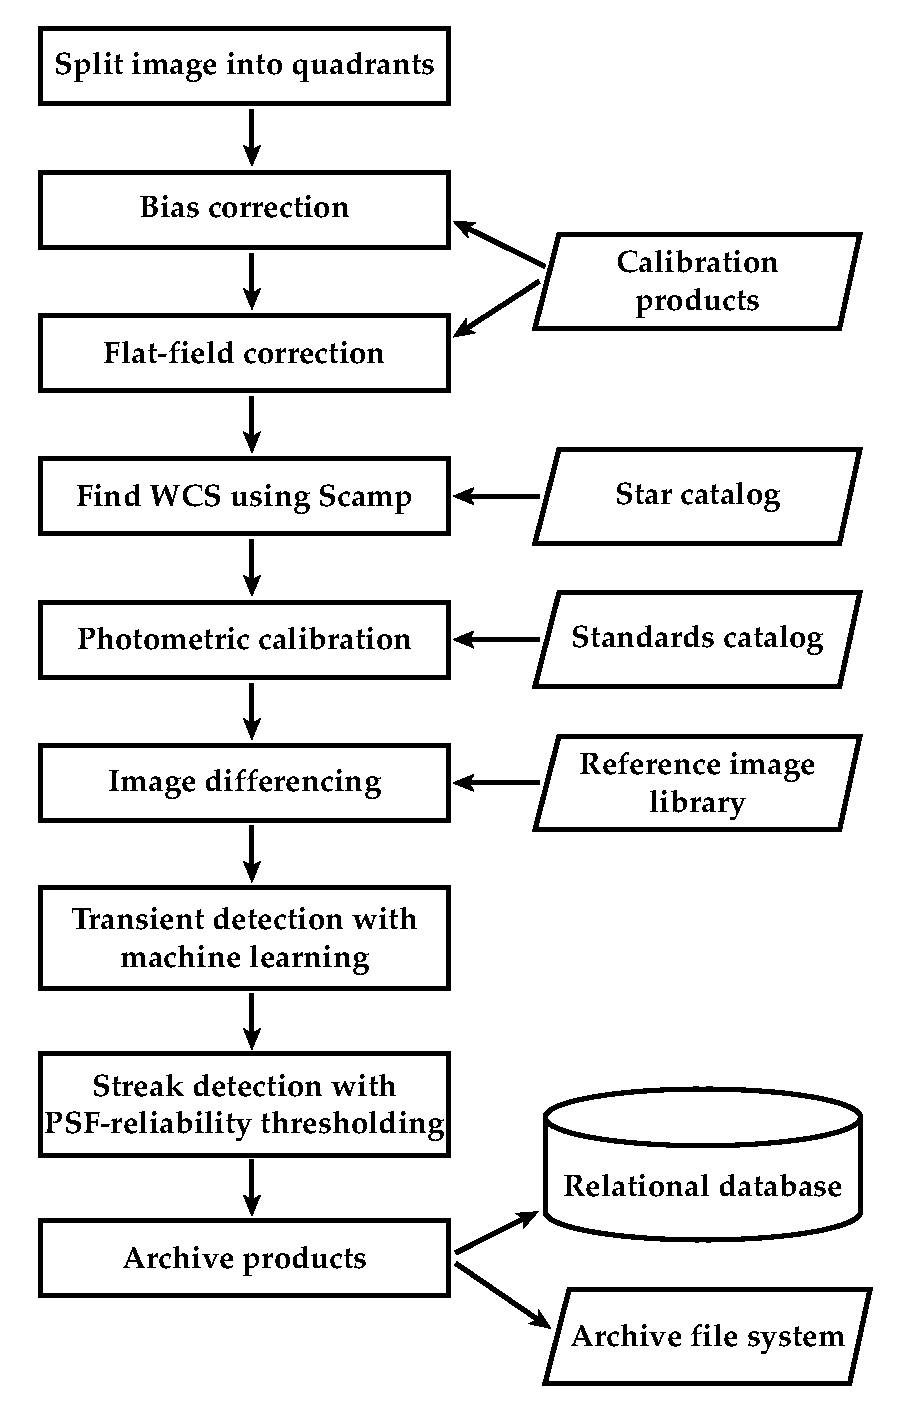
\includegraphics{ztf_calibration_flow}
    \caption[ZTF realtime flowchart]{Flowchart of the ZTF calibration, starting with the raw images on the top and ending with the final science products on the bottom. From \cite{Laher2018}.}
    \labfig{ztf_calibration_flow}
\end{marginfigure}

Each image taken on site (calibration and science exposures alike) is stored as FITS file and subsequently compressed loslessly. The compressed images on average use \SI{5}{\bit} per pixel, so the full image is roughly \SI{380}{\mega\byte} large. These images are immediately sent to IPAC with the High Performance Wireless Research \& Educational Network (HPWREN)\sidenote{\url{https://hpwren.ucsd.edu/}}, a microwave-based data network, linking Palomar Observatory with the IPAC post-processing site. Each transfer typically takes \SI{20}{\second}, keeping up with the pace of ZTF observations \cite{Dekany2020}.

\subsection*{Overscan correction}
As the temperature of the CCDs changes with time, each image is subject to a time-dependent global offset induced by thermal noise. To correct for this, an \textit{overscan} region is used. In the case of the ZTF CCDs, this region does not correspond to physical pixels, but is created during CCD readout. If one reads out more clock cycles then pixels are available, the charge that has gathered during science readout can be accessed. For ZTF, this is done for an additional 24 cycles, corresponding to 24 overscan pixels for each sensor row. After this, the median of these 24 pixels is taken and the full overscan column is fitted with a quadratic function. For each and every image taken by the camera, the bias described by this quadratic function is then subtracted from the image \cite{Masci2019a}.

\subsection*{Bias correction}
The CCD pixels also have different zeropoints. Luckily, this variation has a higher degree of time-stability \sidecite{Howell2006}. To correct it, at the beginning of each night at least 10 so-called \textit{bias} images are taken and overscan corrected. These images are zero-second exposures which are then stacked. After this, the truncated mean of each pixel is calculated, constituting the final bias image for the night (and filter). This bias image is subtracted from each science exposure using the respective filter taken during the night \cite{Masci2019a}.

\begin{marginfigure}
    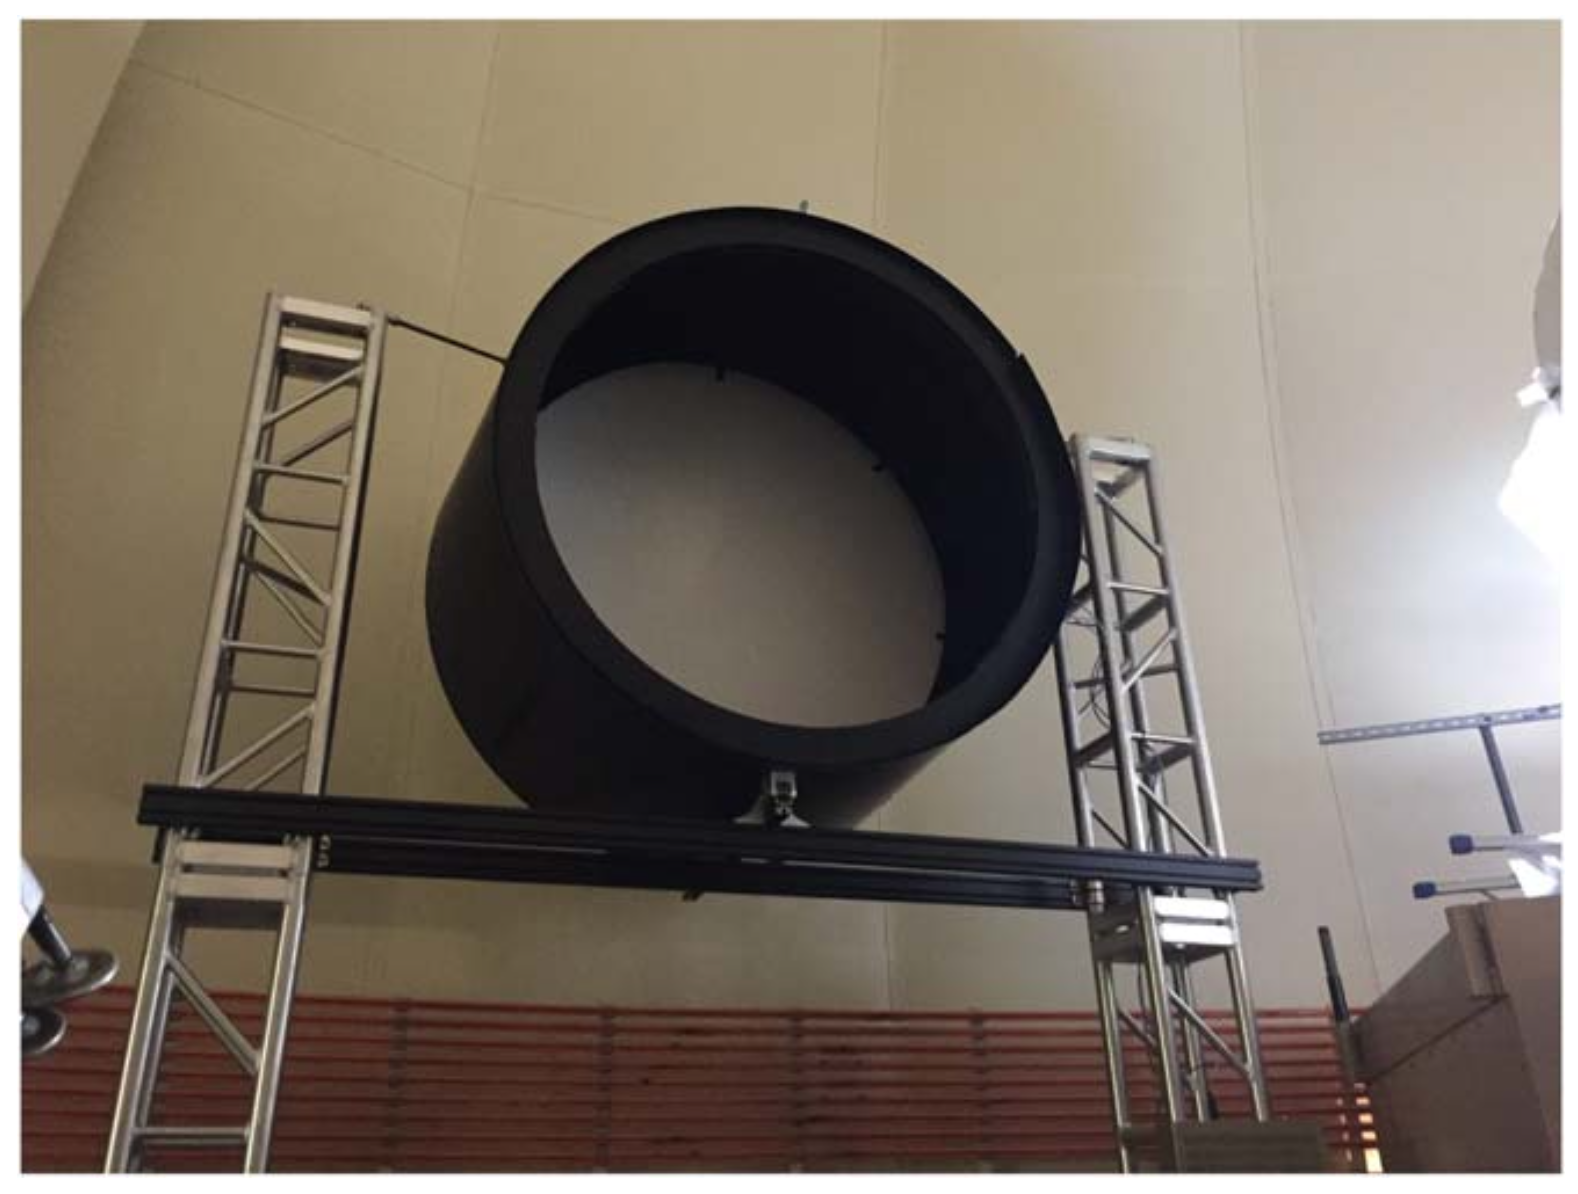
\includegraphics{ztf_flatfield_illuminator.png}
    \caption[ZTF flat field illuminator]{The ZTF flat field illuminator. From \cite{Dekany2020}.}
    \labfig{ztf_flatfield_illuminator}
\end{marginfigure}

\subsection*{Flat fielding}

The pixels in the CCDs do not only differ in zero point, they also have slightly different gain or quantum efficiency. This means, their \textit{response} to light is not uniform. To account for this, the calibration needs a structureless, uniformly bright light source against which the individual pixel response can be measured \cite{Howell2006}. In the case of ZTF this is achieved by using a flat field illuminator consisting of a round screen illuminated by eight identical boards with LEDs, each board housing $4\times15=60$ LEDs of 15 different colors, covering the full wavelength region of ZTF \cite{Dekany2020}.

Each afternoon, before science operations begin, at least 20 images per filter are taken of the flat field illuminator. These are then overscan corrected, the bias image is subtracted, and the pixel values are normalized to a truncated global mean of 1 over the image (to allow for later division). After this individual treatment, all flat field images per filter are stacked to a truncated mean per pixel and outlier rejection is applied to isolate additional noisy pixels. All science images taken during the night are divided by this flat field image \cite{Masci2019a}.

\subsection*{Astrometric calibration}
Astrometric calibration is the mapping of image pixel coordinates to an on-sky coordinate system. For ZTF, this is performed with stars contained in the \textit{Gaia} Data Release 1 (\textit{Gaia} DR1, \sidecite{Brown2016}). As it is a mission designated to high-precision astrometry, \textit{Gaia} is the ideal reference for this task. Prior to cuts, the DR1 contains over 1 Billion sources. From these, sources are selected that are neither too faint, nor run risk of saturating the detector ($12 \leq G \leq 18$ mag). The astrometric solution is derived using the \texttt{SCAMP} \sidecite{Bertin2006} package \sidecite{Masci2019}. For this, stars are extracted with \texttt{SExtractor} \sidecite{Bertin1996} and matched to the \textit{Gaia} stars. The pointing, rotation and polynomial distortion needed to match the stars constitutes the astrometric solution.

\subsection*{PSF photometry} \label{psfphot}
After astrometric calibration, sources in the image need to be extracted to perform photometric calibration (to compare star brightnesses to reference measurements, one first needs stars...). To do so, point spread function (PSF) photometry is employed. Each telescope has a finite aperture, therefore suffering from diffraction. Additionally, earth's atmosphere is constantly and turbulently changing, with different atmospheric layers having different refractive indices, depending on their temperature. This smears out the light from the original point source, an effect known as \textit{seeing} (see Fig. \ref{fig:seeing}).

\begin{figure}[h!]
    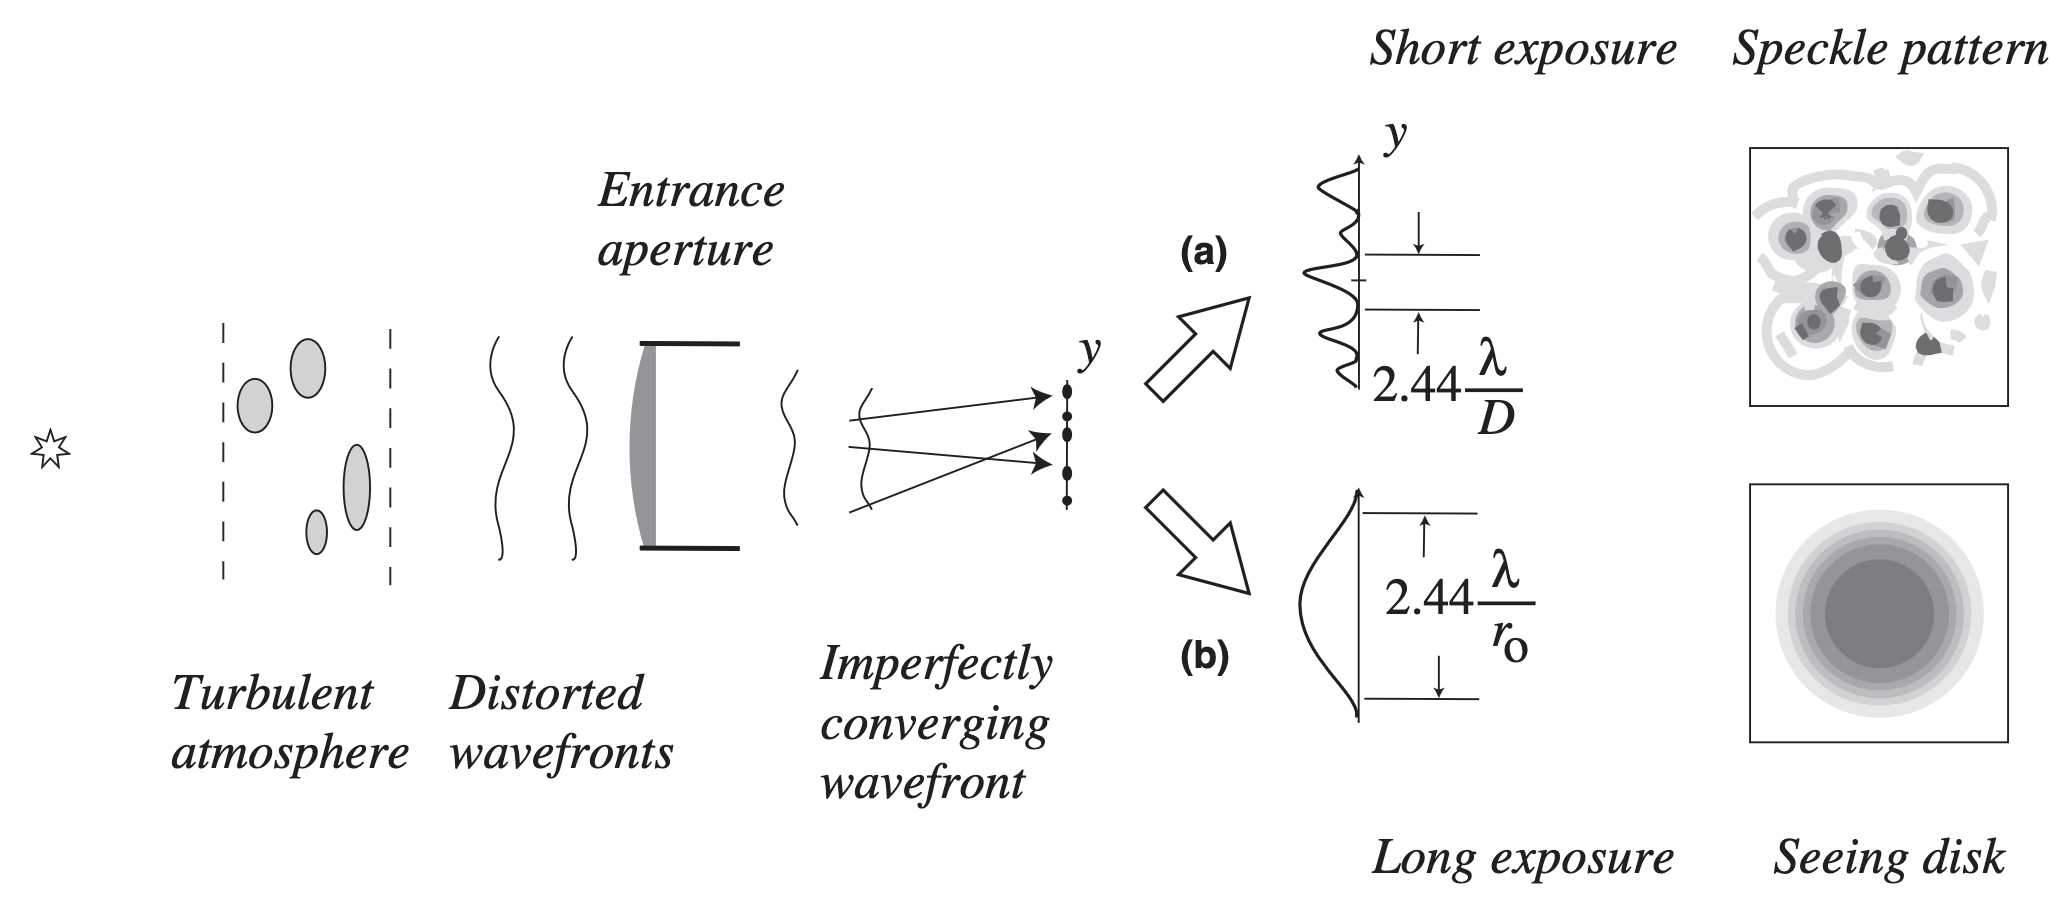
\includegraphics{seeing}
    \caption[Seeing]{\textit{Seeing}: Atmospheric distortions cause time-dependent distortions in the wavefronts, which average out during the exposure and form a Gaussian seeing disk on the sensor (bottom right image). From \cite{Chromey2016}.}
    \labfig{seeing}
\end{figure}

The PSF is describing the way an ideal point source is smeared out spatially after being subjected to atmospheric and optical effects in the telescope, and seeing is the FWHM of the PSF. The algorithm used to reconstruct the PSF of a ZTF exposure is \texttt{DAOphot} \sidecite{Stetson1987}. It fits an analytic Gaussian profile to all point sources within an image. After subtracting this profile, it is iteratively updated with the residuals after subtraction. The background estimate needed for this procedure is extracted from the peak brightness value of a histogram of evenly distributed pixels within the image \cite{Stetson1987}.

\subsection*{Photometric calibration and magnitudes}
\marginnote{Of course, PS1 needs to be calibrated in itself. That is done in two steps: A self-consistent relative calibration is created with \texttt{Ubercal} \cite{Schlafly2012}. This relative calibration is in turn anchored to precisely measured \textit{Calspec} standard stars. For details, see \cite{Magnier2020}}Not only the source positions in the images need to be calibrated (astrometry), but their brightness as well (photometry). To simplify matters, ZTF is photometrically calibrated against a reference survey, namely PS1. To do this, a catalog of useful calibrator stars from the PS1 survey has been curated. These stars are required to fulfill some basic quality criteria: They should be stable over multiple PS1 survey epochs in all PS1 filters excluding the \textit{y}-band (\textit{g}, \textit{r}, \textit{i}, \textit{z}) and should be fairly bright, but not so bright that they saturate the ZTF sensors. Furthermore, they are required to be fairly isolated to avoid blending with neighboring objects and need to have a high probability of being in fact stars (as opposed to galaxies) \cite{Masci2019a}.

The brightness of both ZTF and PS1 are measured in magnitudes. Magnitudes are somewhat counterintuitive, as a higher value corresponds to a fainter source.\sidenote{This can be traced back over 2000 years to Greek/Roman astronomers Hipparchus and Ptolemy \cite{Krisciunas2001}. These classified the brightest stars to be of ``first order'' or ``first magnitude'', with subsequently dimmer stars assigned lower magnitudes until the dimmest stars visible to the naked eye were of ``sixth magnitude''. The system stuck and was put on firm footing by Norman Pogson in 1856. He defined a star being 5 magnitudes brighter than another one to be 100 times brighter \cite{Jones1968}.} The following definition holds:

\begin{definition}
\labdef{magnitude}
A star one magnitude brighter than another star is $\sqrt[5]{100} \approx 2.512$ times brighter
\end{definition}
If one uses flux density (power per unit area) on earth as a measure of brightness, it follows from Def. \ref{def:magnitude} that the difference between two objects with magnitudes $m_1$ and $m_2$ and respective flux densities $f_1$ and $f_2$ is:
\begin{equation}
m_1 - m_2 = -2.5 \log_{10}{\frac{f_1}{f_2}}
\end{equation}
Now we have a \textit{relative} definition of an source's magnitude, but we need an absolute one. In other words, one needs to know what constitutes a magnitude of 0 (the zero point of the magnitude scale). ZTF uses AB magnitudes \sidecite{Oke1983}, which are defined via the spectral flux density $f_\nu$ [\unit{\W\per\m\per\Hz}]. In this sytem, the magnitude is a logarithm of the spectral flux density: 

\begin{definition}
\labdef{abmag_density}
$m_{\text{AB}}(\nu) = -2.5 \log_{10}{(f_\nu/\SI{3631}{\jansky})}$
\end{definition}

As one can see, a source with constant spectral flux density $f_{\nu,0} = \SI{3631e-23}{\W\per\cm\per\Hz} = \SI{3631}{\jansky}$ corresponds to a magnitude of 0.\sidenote{The value of $f_\nu,0$ is not entirely random: The traditional zero point was the star Vega. Vega's magnitude in the AB system as defined above, integrated over the \textit{V}-band, is 0.03, close to the traditional 0. The AB system has the advantage of not relying on a physical source.} Now, telescopes like ZTF and PS1 use bandpass filters, so the spectral flux density is integrated over the filter wavelengths. Therefore, the magnitude definition changes to \sidecite{Tonry2012}:

\begin{definition}
\labdef{abmag}
$m = -2.5 \log_{10}{\frac{\int{f_\nu(h \nu)^{-1}A(\nu)\,d\nu}}{\int{\SI{3631}{\jansky}(h \nu)^{-1}A(\nu)\,d\nu }}}$
\end{definition}
Here, $h$ is Planck's constant and $A(\nu)$ is the capture cross section (i.e. the chance of an incoming photon to produce an electron in the detector\sidenote{More general, $A(\nu)$ is $A(\nu,\theta,t)$, also depending on the angle of the incoming photon and therefore the atmospheric column along the line of sight, as well as time.}). ZTF does not use a precisely modeled response function $A(\nu)$, but relies on PS1. To first order, ZTF magnitudes are tied to the PS1 system via their zero point:

\begin{equation}
m_\text{cal} = m_\text{instr} + \text{ZP}
\end{equation}

To do this, all extracted sources are spatially matched to the PS1 calibrator catalog. After creating a one-to-one relation between ZTF stars and PS calibrator stars, one could to first order calculate $m_\text{cal}$.

But there is a potential complication: The ZTF and PS1 filters are fairly similar, but not exactly so. This means that a celestial object that does not have a constant spectrum (i.e. almost all of them) will have slightly different brightness values when measured with the ZTF and the corresponding PS1 filter. To account for this, a linear, filter-dependent \textit{color correction} $c_f$ needs to be applied:

\begin{equation}
m_\text{cal} = m_\text{instr} + \text{ZP}_f + c_f \times \text{PS1}_\text{clr}
\end{equation}
where $\text{PS1}_\text{clr}$ is filter dependent ($g_\text{PS1}-r_\text{PS1}$ for the ZTF \textit{g}/\textit{r}-band, and $r_\text{PS1}-i_\text{PS1}$ for the \textit{i}-band).

In the photometric calibration step, $\text{ZP}_f$ and $c_f$ are chosen to globally minimize $\Delta m_f = \text{ZP}_f + c_f \times \text{PS1}_\text{clr}$ for all calibrator stars in the respective image \cite{Masci2019a}.

\subsection*{Image subtraction}
Because ZTF is a survey telescope deeply rooted in time-domain astronomy, many of the science goals concern observing sources that are \textit{new} or \textit{changing}. To do so, one needs to detect changes in the nightly observations with regard to \textit{reference images}. From all new images those reference images are subtracted (see Fig. \ref{fig:img_subtraction}). All remaining detections constitute temporal evolution with respect to the epoch of reference image creation. All reference images in ZTF are stacked images of 15--40 individual high-quality images, mostly created while ZTF telescope operations were ramping up\todo{source}. Quality criteria for the individual images comprise good seeing, low errors on the astrometric and photometric calibrations, as well as background levels falling into filter-specific ranges \cite{Masci2019}.

\texttt{SWarp} \sidecite{Bertin2010} is used to interpolate and resample the reference image onto the science image, while subsequent subtraction and PSF photometry (see \nameref{psfphot}) is performed with the \texttt{ZOGY} algorithm \sidecite{Zackay2016}.

\begin{figure}[h!]
    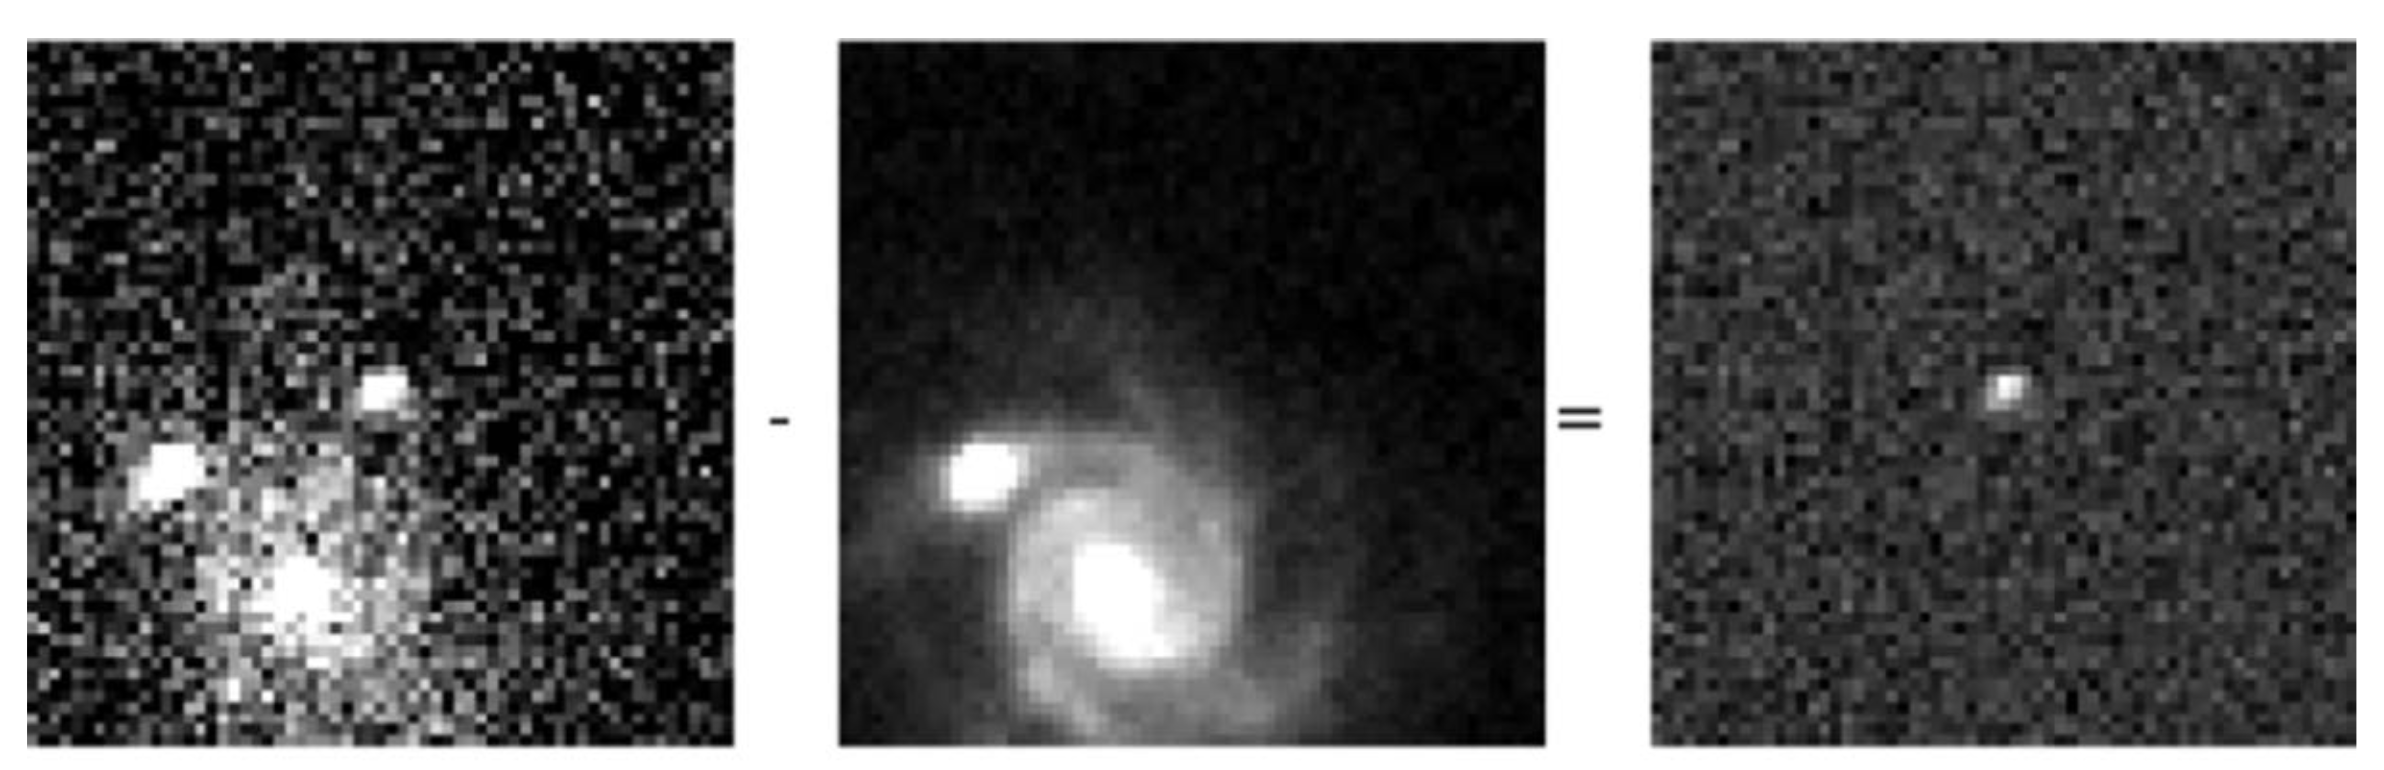
\includegraphics{ztf_imsub.png}
    \caption[ZTF image subtraction]{ZTF image subtraction. The new science image is on the left; in the middle is reference image, which is subtracted. This results in a \textit{difference image}, seen on the right. From \cite{Mahabal2019}.}
    \labfig{img_subtraction}
\end{figure}

\subsection*{Alert packages}
\begin{marginfigure}
    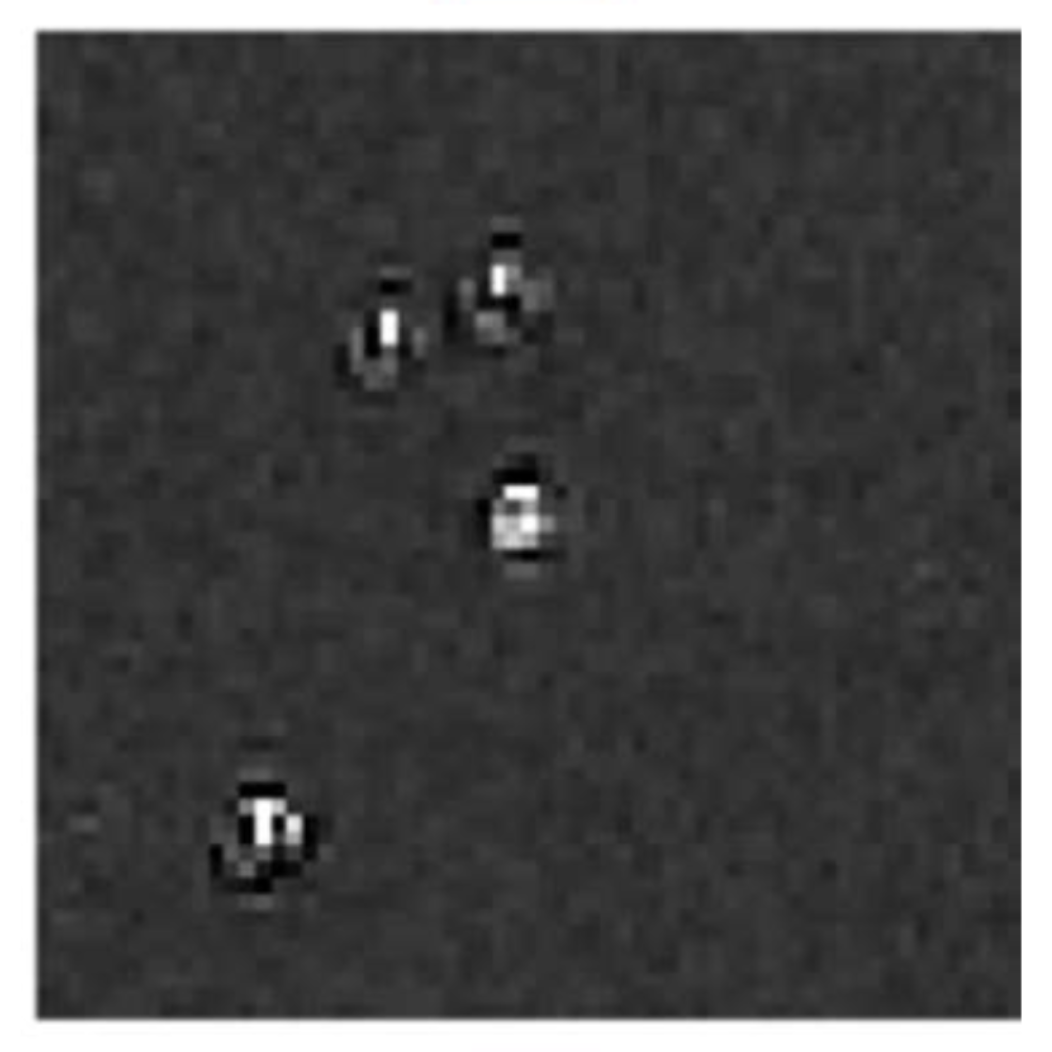
\includegraphics{ztf_bogus.png}
    \caption[ZTF subtraction artifact]{ZTF subtraction artifact, resulting in a bogus transient. From \cite{Mahabal2019}.}
    \labfig{ztf_bogus}
\end{marginfigure}

The last step in the imaging pipeline is alerting an array of upstream transient alert brokers. The information on new transients or updates on existing ones therefore need to be packaged into a convenient format. All positive detections after image subtraction with a signal-to-noise greater than 5 are subjected to a machine-learning (ML) algorithm designated to discriminate between ``real'' (most likely astrophysical) and ``bogus'' (e.g. subtraction artifacts, see Fig. \ref{fig:ztf_bogus}) events \sidecite{Mahabal2019}. This algorithm creates a \texttt{rbscore}, ranking the probability of the detection of being real.

Another ML algorithm has been employed to assign all PS1 sources a \texttt{sgscore}, separating between stars and galaxies based on their morphology and flux in all PS1 bands \sidecite{Tachibana2018}. Both \texttt{rbscore} and \texttt{sgscore}, as well as cutouts of the science, reference and difference images are packed together and shipped as \textit{alert package}. These alerts also include the distances to the three nearest PS1 sources, the closes \textit{Gaia} source, up to 30 days of previous detections if these exist, and some quality metrics like the limiting magnitude. The file format for distribution is Apache Avro\sidenote{\url{https://avro.apache.org}}, and the method of distribution is an Apache Kafka\sidenote{\url{https://kafka.apache.org}} stream \sidecite{Patterson2018}.

\section{Surveys and Cadence}
ZTF is supporting three main survey programs: Firstly, there is the NSF Mid-Scale Innovations Program (MSIP) survey, which is allocated 40\% of telescope time. The MSIP survey is subdivided into the Northern Sky Survey, using a large fraction (85\%) of MSIP time. This survey covers the entire \SI{23675}{\square\deg} of the northern sky \SI{7}{\degree} above the galactic plane. As long as a field (see \nameref{ztf_grid}) is accessible, it is observed once in the \textit{g}- and once in the \textit{r}-band every 3 nights, with both images separated by at least 30 minutes to reject transients and moving (i.e. solar system) objects. The rest of the northern sky ($|b|\leq \SI{7}{\degree}$, with a footprint of \SI{2800}{\square\deg}) is visited twice per night, with the same observational parameters as the Northern Sky Survey \sidecite{Bellm2019a}.